\chapter{Implementation Details}
\label{chap:Implementation Details}
\ffigure{img/implementation.png}{Spatial joins using a simple grid structure. A simple spatial join algorithm that puts elements into buckets based on their position in a grid. By putting data pointers directly in the buckets instead of referring to a linked list, a layer of indirection is removed, and 3-fold improvement is observed. Courtesy of \cite{Sidlauskas2014-ef}.}{fig:implementation}

As we move up the memory hierarchy, careful implementation becomes more important. Recent work by Sidlauskas \ea~claims there is a challenge in concluding about data structures and algorithms only, as the implementation also plays a significant role in performance \cite{Sidlauskas2014-ef}. For instance, if an extra layer of indirection is removed for an algorithm, as seen in Figure \ref{fig:implementation}, we observe a 3-fold performance improvement. 

We have decided to dedicate an entire chapter to \textit{implementation details}, and explain how performance can be improved by reducing the number of branches, avoiding layers of indirection, and utilizing CPU caches.

\newpage

\section{Background Information on Modern CPUs and Compilers}
\label{sec:Background Information on Modern CPUs and Compilers}
Modern processors are capable of performing an enormous amount of calculations per second, but that depends on the amount of available and independent work. The instructions-per-second (IPC) difference between minimal and maximal CPU utilization can easily be an order of magnitude \cite{Boncz2005-wj}. Hence, database software must be implemented such that it fully exploits the processing power made available by the CPU.

\subsection{Pipelining, Superscalar Processing, and Independent Instructions}
\label{sub:Pipelining, Superscalar Processing, and Independent Instructions}
Modern processors improve clock rate and IPC by using a technique known as \textit{pipelining} \cite{Boncz2005-wj}. By dividing an instruction execution into multiple steps, there is less work per stage, and the CPU frequency can be increased. Figure \ref{fig:superscalar} depicts an example pipeline with five stages. However, pipelining also introduce two dangers; \textit{instruction dependencies} and \textit{branch misprediction}.

In a pipeline, \textit{dependencies between consecutive instructions} impose a problem. If an instruction is dependent on another, it must wait for the other instruction to complete before it enters the pipeline. Dependent instructions can severely hurt performance, especially if the pipeline is long.

Dependencies between instructions also relate to conditional branches. When executing a conditional branch instruction, the decision whether to take a branch is usually dependent on the result of a preceding instruction \cite{Boncz2005-wj}. To avoid stalling the pipeline when waiting for the expression to evaluate, modern CPUs use a technique known as branch prediction where the processor immaturely starts executing the branch that is most likely to be taken. The performance penalty occurs if a branch is \textit{mispredicted}, where the instructions in the pipeline must be invalidated (pipeline flushing).

We briefly discussed superscalar processors in Section \ref{sec:Instruction Level Parallelism}. A superscalar processor has multiple execution units to enable IPC $> 1$, and to fully utilize the processor; independent work is required.

\ffigure{img/loop-unrolling.png}{Loop unrolling.}{fig:loop-unrolling}
Hence, to reach maximum performance on a pipelined, superscalar processor, we must find independent work. Since most programming languages do not let the programmer specify which instructions are independent of each other, compiler optimizations play a critical role in CPU utilization \cite{Boncz2005-wj}. The most widely used technique used by the compilers to address this challenge is through \textit{loop unrolling}, which is used to reduce the number of branches and increase independence between functions \cite{Wikipedia_contributors2015-zc}. As seen in Figure \ref{fig:loop-unrolling}, loop unrolling reduces the number of iterations in a loop (reduction of branches) and replaces it with multiple instances of the same instruction. If the instructions are independent, they can be processed in parallel.
\todo{create new figure}

\subsection{CPU Caches}
\label{sub:CPU Caches}
Since transfering data from main memory to CPU can take around $~200$ cycles, modern CPUs utilize multiple layers of on- and off-chip caches to reduce this latency. Efficient usage of caches is paramount for CPU throughput, since roughly 30\% of all instructions in a program are memory loads or stores \cite{Boncz2005-wj}. We know that IPC for DBMSes is strongly impaired by cache misses, and is an important topic for in-memory databases \cite{Exasol2014-xh}.

The best way to tackle this challenge is to design algorithms and data structures that are \textit{cache aware}. Designing such programs is out of the scope of this report, but it briefly boils down to two things:
\begin{itemize}
  \item \textit{Coordinate temporal and spatial locality}. Data processed together should be stored at consecutive memory addresses.
  \item \textit{Avoid false sharing of cache lines}. Multiple cores in a processor should not write to data consecutive in memory at the same time.
\end{itemize}
\textit{Prefetching} is another method used to increase cache performance. Prefetching proactively loads data into caches such that the data is available when an instruction needs it.

\subsection{Call Stack and Subroutine Invocations}
\label{sub:Call Stack and Subroutine Invocations}
\afigure{img/call-stack.png}{A call stack for a program in execution. Each stack frame contains input parameters, function return address, and local variables for a subroutine invocation. Courtesy of \cite{fig:call-stack}.}{fig:call-stack}{0.5}

A \textit{call stack} is commonly used in a computer program to store information and state about active subroutines \cite{Wikipedia_contributors2015-od}. Each time a subroutine is called, a \textit{stack frame} is added to the call stack that stores the input arguments, return address, and variables local to the subroutine. See Figure \ref{fig:call-stack}. The call stack can be implemented in both hardware and software, and the implementation varies between different systems. This stack-based technique implies that calling a subroutine comes at a cost; registers must be stored on the stack, and a new stack frame must be added.

Trading off time with space is usually done to address the above challenge; adding more code to improve program efficiency. \textit{Function inlining} is a technique used by compilers where the subroutine code is copied into the callee's body. This way, the number of stack frames added to the call stack is reduced. \textit{Macro expansion} is a technique that can be applied in several programming languages. Here, multiple copies of function or class definitions are compiled to for instance handle different data types.

\section{Branch Avoidance}
\label{sec:Branch Avoidance}
\ffigure{img/branch-selectivity.png}{Predicate evaluation performance for queries with different query selectivities. A \textit{branch version} and a \textit{predicated version} is tested. For the AthlonMP processor, the branch version are 2-3 times slower on queries with 40\%-60\% selectivites, while the Itanium2 processor has constant processing time. The predicated version offers constant processing time for both processors. Courtesy of \cite{Boncz2005-wj}.}{fig:branch-selectivity}

We saw in the previous section that branches should be avoided due to the penalties of branch misprediction. Besides, branch avoidance might also increase instruction independence.

An example of the consequences of inaccurate branch prediction is studied by Neumann \ea~\cite{Neumann2011-uq}. In this research, the performance of queries with various selectivities were tested. As we can see in Figure \ref{fig:branch-selectivity}, queries with 40\%-60\% selectivity executed on an AthlonMP processor are roughly 2-3 times slower than queries with selectivities close to 0\% or 100\%. The Itanium2 processor does not have the same characteristic, as the Itanium architecture allows for both \textit{not taken} and \textit{taken} branches to be executed simultaneously.

Neumann \ea~also developed a branchless version (predicated version) to evaluate predicates in the queries. The branchless variant is denoted as \texttt{/* predicated version */} in Figure \ref{fig:branch-selectivity}. For both AthlonMP and Itanium2 processors, this implementation offers constant performance for all selectivities, but is, in general, more expensive.

Branch avoidance is also important in other parts of the system, like decompressing. Zukowski \ea~present a decompression algorithm that is free for \textit{if-then-else} statements \cite{Zukowski2006-oz}. By running the algorithm in two tight loops instead of one, branch misprediction is reduced, and the loops can be pipelined by a compiler.

Branches can also be avoided by compiling queries to machine code \cite{Lamb2012-kg}. We study this technique in greater detail in Section \ref{sub:Compiling Queries Into Machine Code}.

\subsection{Short-circuiting}
\label{sub:Short-circuiting}
\missingfigure{Consider putting in a figure about short circuiting here}
\textit{Short circuiting} is referred to a special case of Boolean operator evaluation in which the next argument is not evaluated if the current argument is sufficient to determine the value of the expression \cite{Wikipedia_contributors2015-rk}. An example from the database world is if the first predicate is false, the following predicates is never evaluated as the record will never become a part of the record set. Short circuit boolean operators not simple arithmetic operators, but a control structure.

Since short-circuit boolean operators are control structures and not simple arithmetic operators, there is a chance of branch misprediction. That is why \blink~\cite{Raman2008-gi, Johnson2008-cp} does not short circuit between tuples. If a block is selected for scanning, all fields in a record are checked, and the result is a candidate vector. Short circuiting only improves performance on low selectivity queries.

\section{Cache awareness}
\label{sec:Cache awareness}
In addition to avoiding branches and optimizing for loop pipelining, the implementation must also be aware of the computer cache. The CPU caches are important, since 30\% of the instructions given to the CPU are loads and stores \cite{Boncz2005-wj}. There are multiple ways to go about cache awareness. The developers behind \exasol claims that high level of data locality is one of the key factors for performance \cite{Exasol2014-xh}.

Perhaps the most important, is that algorithms must be cache aware \cite{Farber2012-vh}. In terms of database algorithm, several cache aware variants have been proposed. \monetdb~\cite{Boncz2002-yj} introduce a clever clustering algorithm called \term{radix cluster}, where cache utilization is maximized by performing muliple passes over the data. \oracle~\cite{Lahiri2015-mz} uses an algorithm known as \term{Vector Group By}, which is a compact multidimensional array for storing aggregate results.

Not only is data locality important, but also code locality \cite{Neumann2011-uq}. When compiling queries into code, there is a question of code size versus function definitions. If no functions are generated, there is an exponetial growth of code. Therefore, a balance must be found, but the important thing is that a hot path never cross a function boundary.

\subsection{Prefetching}
\label{sub:Prefetching}
Prefetching is the act of getting data up the storage hierarchy before the data is actually needed. Prefetching is made available to the processors if vectorized execution is used. Explicit prefetching is used by several systems, like \ibm~\cite{Raman2013-em}, \monetx~\cite{Boncz2005-wj}. \exasol uses special CPU instructions to prefetch certain memory locations to improve data locality \cite{Exasol2014-xh}.

\subsection{How to get cache awareness}
\label{sub:How to get cache awareness}
First of all, cache locality is improved by using compression \cite{Lemke2010-is}, which is described in Chapter \ref{chap:Compression}.

Secondly, vectorized execution increases cache behavior \cite{Larson2013-mc}.
\section{Loop Pipelining and Vectorized Execution}
\label{sec:Loop Pipelining and Vectorized Execution}
The absence of loop pipelining can have dramatic effects on query performance. Boncz \ea~\cite{Boncz2005-wj} show how the \mysql uses 49 cycles per tuple due to the absence of loop pipelining.

In order to ensure proper loop pipeline behavior, compilers must know that pointers do not overlap, such that loop unrolling can be used. CPU primitives expose to the compiler that processing a tuple is independent from the others. This is also important in the decompression and compression step \cite{Zukowski2006-oz}

A simple technique is presented by Zukowski \ea~\cite{Zukowski2006-oz} is the \term{Two pointer solution}, where you use two pointers in a loop instead of one, and cut the number of iterations in half.

Loop pipelining is studied as vectorized execution in Section \ref{sec:Vectorized Execution}

\subsection{Vectorized Execution}
\label{sub:Vectorized Execution}
We round off this chapter by explaining a query technique that helps all three, namely vectorized execution.

Vectorized execution is processing the queries by processing multiple rows (vectors) at the same time, and therefore avoid tuple-at-a-time processing. The benefits from this is investigated in \cite{Abadi2008-dd}, and it increases performance by 50\% on average \todo{check this out}. Vectorized execution enables loop unrolling, memory prefetching, and minimizing of cache misses \cite{Larson2013-mc}. In other words, vectorized execution will boost the above points (Branch avoidance, loop pipelining, and cache awareness).

Vectorized execution is used by many systems out there. \ibm~\cite{Raman2013-em} works on thousands of row at a time. \mssql~\cite{Larson2013-mc} works on thousands of rows in a batch. The result of each block is a row vector that indicates whether a row has been logically purged from the batch. \monetx~\cite{Boncz2005-wj} uses vectors as their main structure, which is the basic construct that is passed around. Zukowski \ea~\cite{Zukowski2006-oz} proose a vectorized query engine, and branching overhead is reduced due to only one function call per vector.

By processing vectors at a time, data flow is coupled to control flow \cite{Stonebraker2005-qz, Lamb2012-kg}.

In terms of vector size, the vector should not be too small (no paralellism), nor too big, as it must fit in cache \cite{Boncz2005-wj}

However, there are certain drawbacks by using vectorized execution. The research of Neumann \ea~\cite{Neumann2011-uq} indicates that pipelining is harder, since data must be materialized to memory from one step to the next, instead of residing in the CPU registers.

The vectorized execution model comes as a contrast to the \term{Volcano} like execution model, where computations and aggregations are all done in a single pass. This is used in \monetx, where small vertical chunks of cache-resident data are the unit of operation \cite{Boncz2005-wj}. This model is nice an simple, but is primarily built when I/O was the major bottleneck \cite{Neumann2011-uq}.

\section{Avoding Layers of Indirection}
\label{sec:Avoding Layers of Indirection}

\subsection{Macro expansions}
\label{sub:Macro expansions}
To avoid branches and exploin loop pipelining, two techniques are used. The first one is to use macro expansions when developing the database. \monetdb~\cite{Boncz2002-yj} uses macro expansions such that multiple functions per operator are compiled for different data types. All

\subsection{Compiling into machine code}
\label{sub:Compiling into machine code}
\begin{figure}
  \centering
  \begin{subfigure}{0.45\textwidth}
    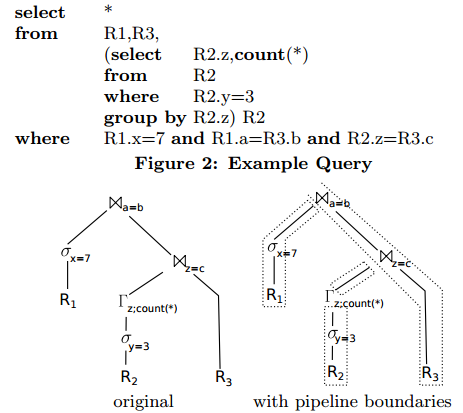
\includegraphics[width=\textwidth]{img/pipeline-boundary-1.png}
    \caption{...}
    \label{fig:pipeline-boundary-1} 
  \end{subfigure}
  \begin{subfigure}{0.45\textwidth}
    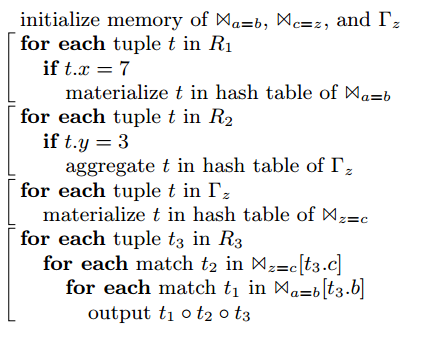
\includegraphics[width=\textwidth]{img/pipeline-boundary-2.png}
    \caption{...}
    \label{fig:pipeline-boundary-2} 
  \end{subfigure}
  \caption{Pipeline boundaries. Courtesy of \cite{Neumann2011-uq}.}
  \label{fig:pipeline-boundary} 
\end{figure}
The work by Neumann \ea~\cite{Neumann2011-uq} explains how queries are compiled into native machine code using the LLVM compiller framework. Doing this, the processing of queries are data centric and not operator centric. Classical query processing always wipes the CPU registers, but in their solution they push tuple values until a pipeline is broken. They tried using the C++ compiler, but it turned out too slow. Therefore, the major application was developed in C++. According to the developers behind the \hyper~database, compilation of queries will increase the performance of ad-hoc queries because ...

The technique of compiling queries and data structures are used by several databases. \blink~\cite{Barber2012-xt}, \ibm~\cite{Raman2013-em}, \vertica~\cite{Lamb2012-kg} generates a different code per frequency partition, since the dictionaries are different. 


In terms of application specific compliation, it is not only a question of precompiling the queries, but also compiling the column stores and other data structures directly. \mssql~\cite{Delaney2014-ip} memory database are natively compiled into DLLs and queries and stored procedures are run as native code.\qlikview~\cite{noauthor_undated-js} data is compiled straight into machine code, and temporary toolkup tables are used. They claim a performance increase of 10\%.





\section{Chapter Conclusion}
\label{sec:Chapter Conclusion}

